\PassOptionsToPackage{quiet}{fontspec}
\documentclass[12pt,a4paper,UTF8]{article}
\usepackage{thesis} % 格式控制
\setlength{\parindent}{2em} % 控制首行缩进  
\addtolength{\parskip}{3pt} % 控制段落距离  
\onehalfspacing % 1.5倍行距  
\graphicspath{{./figures/}} % 指定图片所在文件夹  
\usepackage{svg}


\classname{智能控制技术}  % 设置课程名称
\makepagestyle{递阶控制}{\printclassname ~实验报告}




\begin{document}
\maketitlepage{递阶控制}{教7-306}{PhilFan}{19260817}{\today}{刘山} %封面页 



\begin{figure}[hbtp]
    \centering
    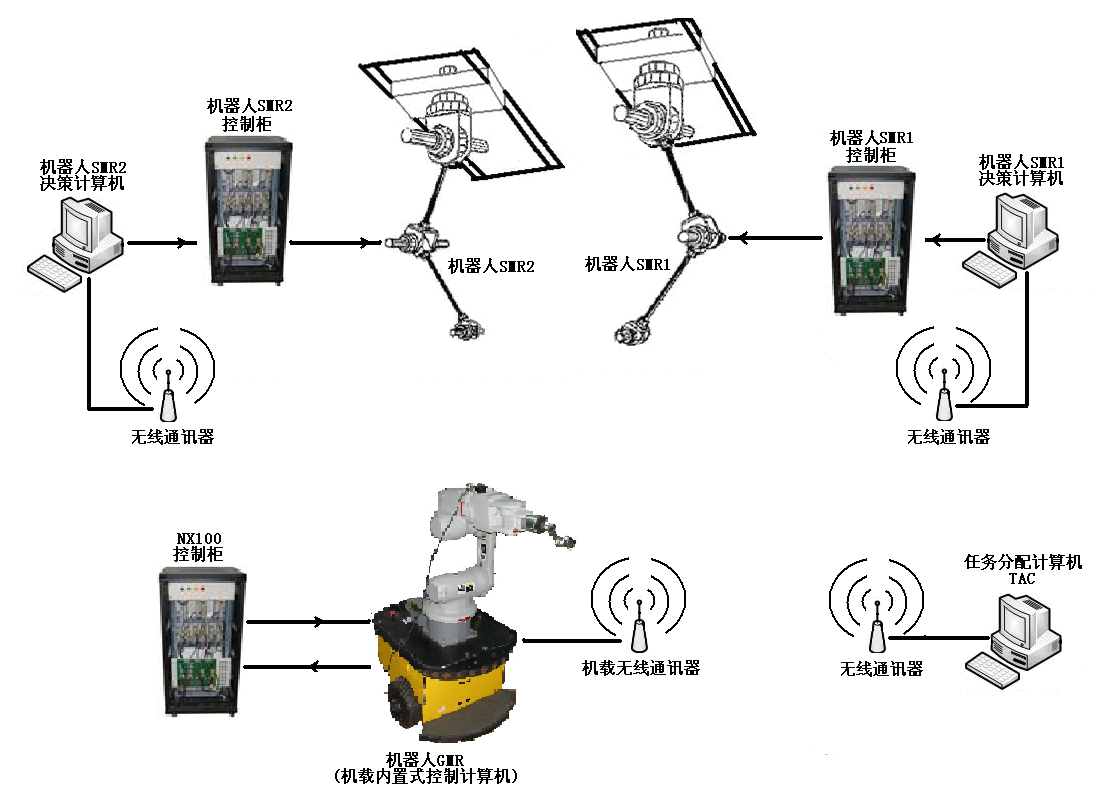
\includegraphics[width=\linewidth]{figures/1.png}
\end{figure}


\begin{problem}
如图所示的多机器人协作系统由三个机器人组成,分别为两个悬挂移动式多关节机器人(SMR1和SMR2)和一个地面移动式多关节机器人(GMR)。

SMR1和SMR2的主体是两个七关节式机器人,悬挂在一个固定在顶部的方形托架上,它们的移动支架都能够沿着悬挂导轨在方形托架的允许范围内移动。GMR的主体是六关节式机器人HP3,安装在一个轮式移动基座PowerBot上,能够在地面上随意移动。

系统配置三级视觉系统,第一级为全局的外部三维点云相机,第二级为装在机械臂腕部的深度相机,第三级为装在机械臂手抓中心的摄像头。各机械臂均配备力矩传感器。

SMR1、SMR2和GMR都有自己独立的控制计算机,系统中另有一台独立的计算机TAC,各计算机之间通过无线通讯连接,实现数据交互。

系统的目标任务是:从无序堆放的工件中拾取目标螺杆,并将螺杆的两端装上合适的螺帽,然后放置在期望目标位置。

请根据以上各部分的具体任务和功能,采用递阶控制的思想将多机器人协作系统进行分解,并画出该递阶控制系统的分级系统结构图。

\end{problem}

\begin{figure}[htbp]
    \centering
    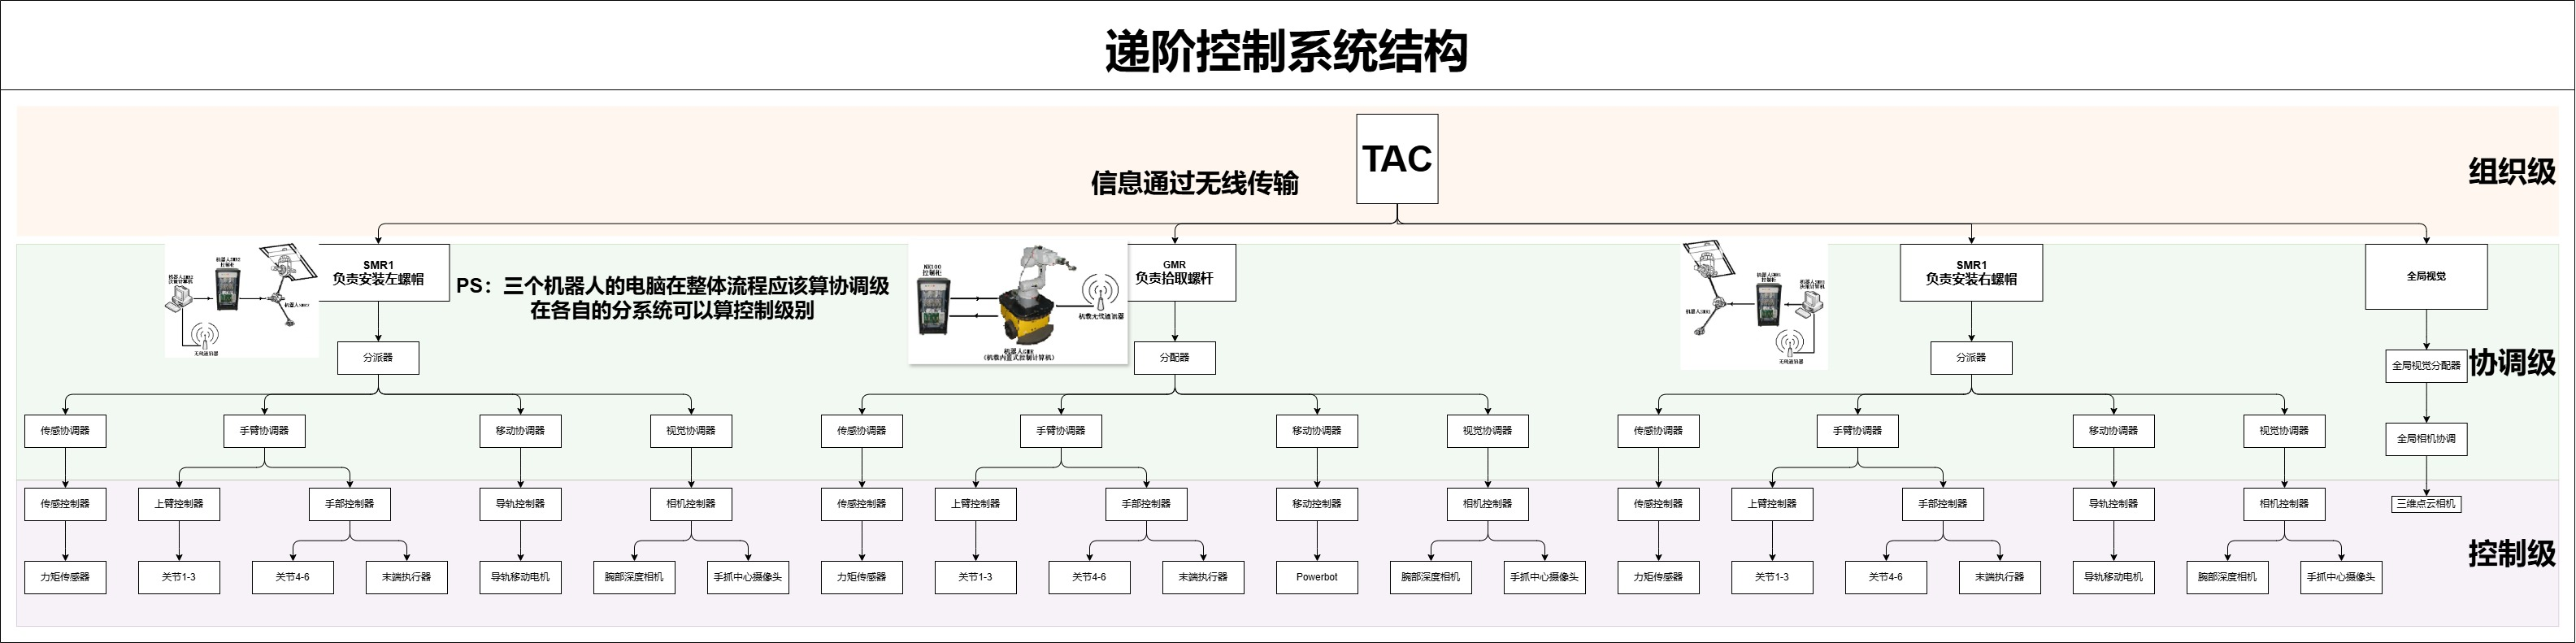
\includegraphics[width=1\linewidth]{figures/hw01.jpg}
\end{figure}

因为pdf中不太好插入太大的图片,我将高清版图片作为附件一并提交了。


\section{设计原则}

\begin{itemize}
    \item \textbf{组织级}:精度较低,但具有较高的智能决策能力,基于复杂的人工智能技术进行任务规划与分配。决策过程涉及高层次的推理、规划和优化,任务复杂度较高。
    \item \textbf{协调级}:精度逐步提高,智能相对减少。此级通过神经模糊网络或Petri网等工具,实现任务协调和控制信号优化,确保任务按照组织级指令进行精细调整。
    \item \textbf{执行级}:精度最高,智能最低。执行级依靠精确的控制理论(如PID控制、神经网络控制等)来确保每个机器人执行任务的高精度操作。
\end{itemize}

\begin{itemize}
    \item \textbf{知识流量}:通过不同层级之间的信息传递与反馈,不同层级的熵会影响系统的工作能力。在此过程中,执行级的低智能、高精度操作与组织级的高智能、低精度决策形成对比,帮助实现任务的有效分配和执行。
    \item \textbf{熵(Entropy)}:系统中的每个层级有不同的熵值,组织级的熵较高(代表信息量大且决策复杂),执行级的熵较低(控制精度高但任务较简单)。通过精度递增和智能递减的方式,系统总体熵最小化,确保任务高效完成。
\end{itemize}

这种递阶智能控制结构使得多机器人协作系统能够高效、精确地执行复杂任务,并在不同层级间实现智能与精度的平衡,最大化系统的工作能力。


\section{组织级(顶层)}
\begin{itemize}
    \item \textbf{目标任务}:从无序堆放的工件中拾取目标螺杆,装配螺帽并放置到期望位置。
    \item \textbf{控制目标}:
    \begin{itemize}
        \item \textbf{规划与决策}:基于高级人工智能与专家系统,制定任务的总体规划。
        \item \textbf{任务分配}:从视觉系统:外部三维点云相机,根据每个机器人的能力和位置,将任务分配给SMR1、SMR2和GMR。
    \end{itemize}
    \item \textbf{技术应用}:
    \begin{itemize}
        \item 专家系统与推理技术,用于任务分配和全局决策。
        \item 可能使用\textbf{模糊逻辑}或\textbf{Boltzmann机}等方法进行决策优化。
    \end{itemize}
\end{itemize}

\section{协调级(中层)}
\begin{itemize}
    \item \textbf{控制目标}:
    \begin{itemize}
        \item \textbf{任务协调}:接收组织级的高层指令,协调各机器人执行的子任务。
        \item \textbf{优化控制器设定}:根据执行级反馈的信息,优化每个机器人的控制参数和执行策略。
        \item \textbf{信息流与状态更新}:确保机器人状态和执行结果能传回组织级进行决策优化。
    \end{itemize}
    \item \textbf{技术应用}:
    \begin{itemize}
        \item \textbf{Petri网}和\textbf{神经模糊网络}:用于协调任务和优化控制信号。
        \item \textbf{与或图}、\textbf{状态空间}技术帮助规划机器人的协作流程。
    \end{itemize}
\end{itemize}

\section{执行级(底层)}
\begin{itemize}
    \item \textbf{控制目标}:
    \begin{itemize}
        \item \textbf{精确控制}:执行精确的机器人操作,包括关节运动控制、抓取和装配等。
        \item \textbf{实时反馈}:通过力矩传感器和视觉传感器获取实时数据,调整控制指令。
    \end{itemize}
    \item \textbf{技术应用}:
    \begin{itemize}
        \item \textbf{神经网络}或\textbf{PID控制}:作为机器人控制器,执行协调级提供的控制信号,精确控制每个机器人的运动和任务执行。
    \end{itemize}
    \item \textbf{控制器与传感器}:
    \begin{itemize}
        \item \textbf{关节控制器}:精确控制机械臂的各个关节运动。
        \item \textbf{力矩传感器}:实时监测机器人在抓取螺杆和装配螺帽时的力反馈,确保操作过程的稳定性。
        \item \textbf{导轨移动电机}:控制SMR1和SMR2的移动,确保其在轨道上沿规定路径精确移动。
        \item \textbf{PowerBot控制器}:负责地面机器人GMR的运动控制,通过轮式移动基座进行任务搬运。
        \item \textbf{腕部深度相机}:提供精确的视觉信息,帮助机器人定位螺杆及其位置。
        \item \textbf{手抓中心摄像头}:为机器人提供抓取目标的实时图像数据,确保装配精度。
    \end{itemize}
\end{itemize}






\end{document}
